
\begin{figure}[H]
    Mezi uzly \(V_{CC}\) a \(GND\) je umístěn napěťový zdroj s napětím \(V_{CC} = 1.8 [V]\), pro zjednodušení jen není uveden ve schematu, což bude platit i u dalších zapojení.

    \vspace{8mm}
    \begin{minipage}{0.5\textwidth}
        \begin{circuitikz}[scale=1, transform shape] 
            \draw
              % MOSFET transistor with labels for drain (D), gate (G), source (S), and bulk (B)
              (0,0) node[nmos, bulk] (mos) {}
              (mos.drain) node[left] {M1}
            
              % Gate voltage source VGS
              (mos.gate) to[short, -] ++(-2,0) to[voltage source, l^=$V_{GS}$] ++(0,-1.5) node[ground] {}
              
              % Drain voltage source VDS (vertical)
              (mos.drain) to[short, -] ++(0,1) -- ++(2,0) -- ++(0,-1) to[voltage source, l^=$V_{DS} $] ++(0,-2) -- (2,-1.5) node[ground] {}
              
              % Source connected to ground, aligned with VGS ground
              (mos.source) to[short, -] (0,-1.5) node[ground] {}
              
              % Bulk (body) connection to ground
              (mos.bulk) to[short, -] (0.5, 0) -- ++(0,-1) -- ++(-0.5,0)  node[circle,fill,inner sep=1.2pt] (myNode) {}
            ;
        \end{circuitikz}

        \vspace{5mm}
        \centering{(NMOS)}
    \end{minipage}
    \hfill
    \begin{minipage}{0.5\textwidth}
        \begin{circuitikz}[scale=1, transform shape] 
            \draw
                % MOSFET transistor with labels for drain (D), gate (G), source (S), and bulk (B)
                (0,0) node[pmos, bulk] (mos) {}
                (0.5,0) node[right] {M1}
            
                % Gate voltage source VGS
                (mos.gate) to[short, -] (-2,0) to[voltage source, l^=$V_{GS}$] (-2,2) -- ++(2,0) -- (mos.source)
                
                % Drain voltage source VDS (vertical)
                (mos.drain) to[short, -] (0,-1) to[voltage source, l^=$V_{DS} $] ++(0,-1) node[ground] {}
                
                % Bulk (body) connection to ground
                (mos.bulk) to[short, -] (0.5, 0) -- ++(0,1) -- ++(-0.5,0)  node[circle,fill,inner sep=1.2pt] (myNode) {}

                % VCC
                (0,2)  to[short, *-o] ++(1,0) node[above, right]{$V_{CC}$}
            ;
        \end{circuitikz}

        \vspace{5mm} 
        \centering{(PMOS)}
    \end{minipage}
    \caption{\label{cod:cod_NP_WL_const} Zapojení pro určení závislosti modulace delky kanálu \(\lambda\) na delce kanálu \(L\)}
\end{figure}

\begin{lstlisting}[language=Spice, caption={ \centering Kod simulace použítí pro získání závislosti \\ modulované délky kanálu \(\lambda\) na délce kanálu \(L\)}, label={cod:cod_lambda}]
.lib cmos018.txt
.step param lset 0.1u 10u 0.02u
.param wset=9.2*lset ; pro PMOS
.param wset=2.3*lset ; pro NMOS
.meas DC ID1 FIND Id(M1) WHEN V(VD)=0.5
.meas DC ID2 FIND Id(M1) WHEN V(VD)=1.3
.meas DC ID0 FIND Id(M1) WHEN V(VD)=0.9
.meas rout param (1.3-0.5)/(ID2-ID1)
.meas lambda param 1/(ID0*rout)
.dc UDS 0.5 1.3 10m
\end{lstlisting}

\begin{figure}[H]
    \centering
    \begin{tikzpicture}
        \begin{axis}[
            xlabel={Delka kanálu \(L [\mu m]\)},
            ylabel={Modulované délky kanálu \(\lambda\)},
            grid=major,
            width=0.8\linewidth,
            height=0.4\linewidth,
            ytick distance=0.1,
            xmin=0, xmax=10,
            ymin=0, ymax=0.7,
            legend pos=north east           
        ]
        \addplot table [
            x=L,
            y=lambda, 
            col sep=comma,
            mark=none
        ] {data/lambdaNMOS.csv};
        \addlegendentry{NMOS}
        \addplot table [
            x=L,
            y=lambda,
            col sep=comma,
            mark=none
        ] {data/lambdaPMOS.csv};
        \addlegendentry{PMOS}
        \end{axis}
    \end{tikzpicture}
    \caption{Závislost \(U_{TH}\) na napětí bulku}
    \label{fig:lambda}    
\end{figure}

\begin{figure}[H]
    \vspace{8mm}
    \begin{minipage}{0.5\textwidth}
        \begin{circuitikz}[scale=1, transform shape] 
            \draw
              % MOSFET transistor with labels for drain (D), gate (G), source (S), and bulk (B)
              (0,0) node[nmos, bulk] (mos) {}
              (mos.drain) node[left] {M1}
            
              % Gate voltage source VGS
              (mos.gate) to[short, -] ++(-2,0) to[voltage source, l^=$V_{GS}$] ++(0,-1.5) node[ground] {}
              
              % Drain voltage source VDS (vertical)
              (mos.drain) to[short, -] ++(0,1) -- ++(2,0) -- ++(0,-1) to[voltage source, l^=$V_{DS} $] ++(0,-2) -- (2,-1.5) node[ground] {}
              
              % Source connected to ground, aligned with VGS ground
              (mos.source) to[short, -] (0,-1.5) node[ground] {}
              
              % Bulk (body) connection to ground
              (mos.bulk) to[short, -] (0.5, 0) -- ++(0,-1) -- ++(-0.5,0)  node[circle,fill,inner sep=1pt] (myNode) {}
            ;
        \end{circuitikz}

        \vspace{5mm}
        \centering{(NMOS)}
    \end{minipage}
    \hfill
    \begin{minipage}{0.5\textwidth}
        \begin{circuitikz}[scale=1, transform shape] 
            \draw
              % MOSFET transistor with labels for drain (D), gate (G), source (S), and bulk (B)
              (0,0) node[pmos, bulk] (mos) {}
              (mos.drain) node[left] {M1}
                          
              % Gate voltage source VGS
              (mos.gate) to[short, -] (-2,0) to[voltage source, l^=$V_{GS}$] (-2,2) -- ++(2,0) node[circle,fill,inner sep=1pt] (myNode) {}
              
              % Drain voltage source VDS (vertical)
              (mos.source) to[short, -] (0,2) -- ++(2,0) -- ++(0,-1) to[voltage source, l^=$V_{DS} $] ++(0,-2) -- (2,-1.5) -- (0,-1.5)
              
              % Source connected to ground, aligned with VGS ground
              (mos.drain) to[short, ] (0,-1.5) node[circle,fill,inner sep=1pt] (myNode) {} (0,-1.5) node[ground] {}

              % Bulk (body) connection to ground
              (mos.bulk) to[short, -] (0.5, 0) -- ++(0,1) -- ++(-0.5,0)  node[circle,fill,inner sep=1pt] (myNode) {}

            %   (2,2)  to[short, *-o] ++(1,0) node[above, right]{$V_{CC}$}
            ;
        \end{circuitikz}

        \vspace{5mm} 
        \centering{(PMOS)}
    \end{minipage}
    \caption{\label{cod:cod_NP_WL_const} Zapojení pro určení závislosti modulace delky kanálu \(\lambda\) na delce kanálu \(L\)}
\end{figure}

\begin{lstlisting}[language=Spice, caption={ \centering Kod simulace použítí pro získání závislosti \\ modulované délky kanálu \(\lambda\) na délce kanálu \(L\)}, label={cod:cod_lambda}]
.lib cmos018.txt
.step param lset 0.1u 10u 0.02u
.param wset=5*lset
.meas DC ID1 FIND Id(M1) WHEN V(VD)=0.5
.meas DC ID2 FIND Id(M1) WHEN V(VD)=1.3
.meas DC ID0 FIND Id(M1) WHEN V(VD)=0.9
.meas rout param (1.3-0.5)/(ID2-ID1)
.meas lambda param 1/(ID0*rout)
.dc UDS 0.5 1.3 10m
\end{lstlisting}

\vspace{-7mm}
\begin{figure}[h]
    \centering
    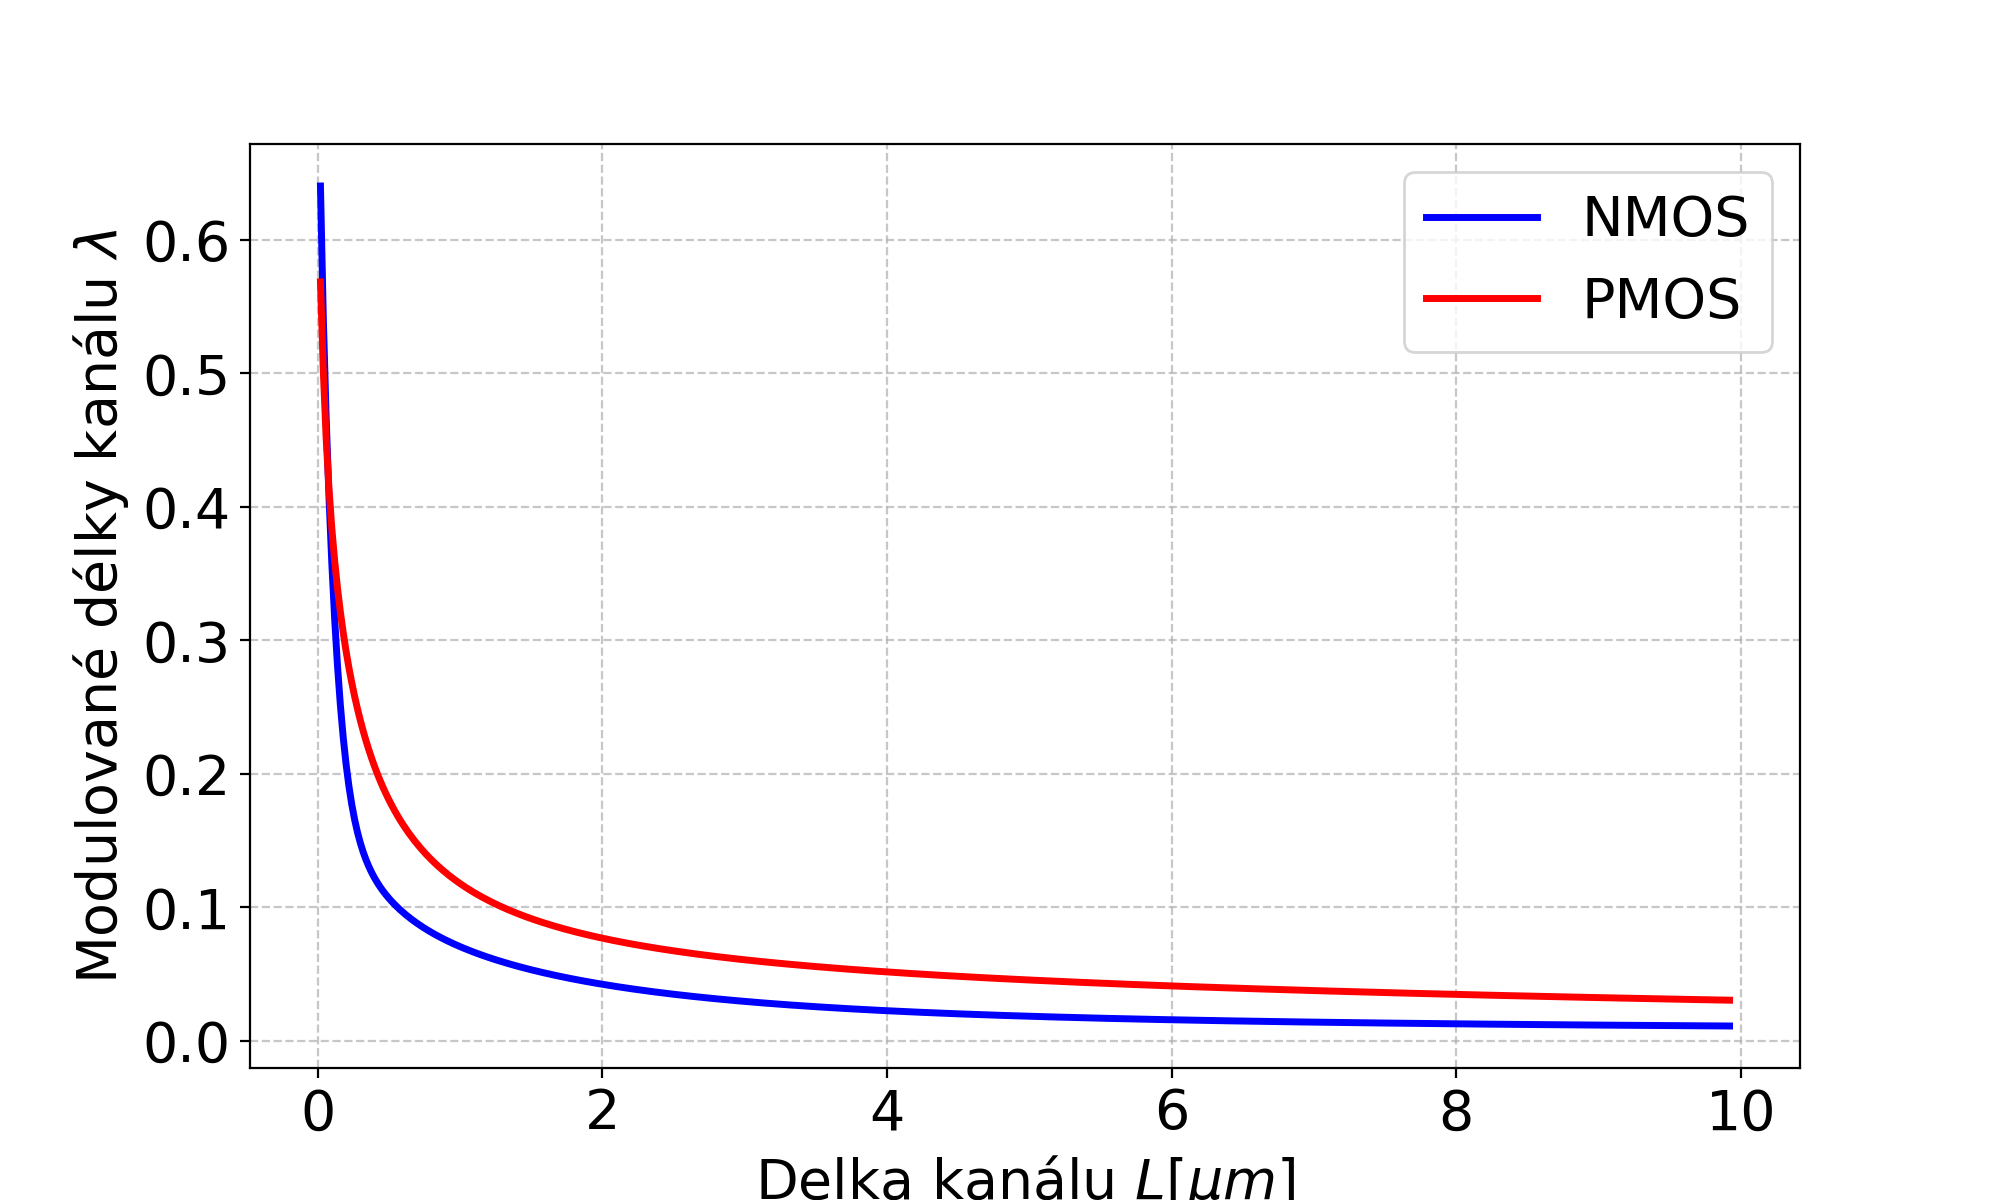
\includegraphics[height=0.28\textheight]{text/img/lambda.png}
    \caption{\label{fig:lambda} Závislost parametru \(\lambda\) na délce kanálu \(L\) při poměru \(W/L = 5\)}
\end{figure}

\vspace{-1mm}
\begin{figure}[H]
    \vspace{8mm}
    \begin{minipage}{0.5\textwidth}
        \begin{circuitikz}[scale=1, transform shape] 
            \draw
              % MOSFET transistor with labels for drain (D), gate (G), source (S), and bulk (B)
              (0,0) node[nmos, bulk] (mos) {}
              (mos.drain) node[left] {M1}
            
              % Gate voltage source VGS
              (mos.gate) to[short, -] ++(-2,0) to[voltage source, l^=$V_{GS}$] ++(0,-1.5) node[ground] {}
              
              % Drain voltage source VDS (vertical)
              (mos.drain) to[short, -] ++(0,1) -- ++(2,0) -- ++(0,-1) to[voltage source, l^=$V_{DS} $] ++(0,-2) -- (2,-1.5) node[ground] {}
              
              % Source connected to ground, aligned with VGS ground
              (mos.source) to[short, -] (0,-1.5) node[ground] {}
              
              % Bulk (body) connection to ground
              (mos.bulk) to[short, -] (0.5, 0) -- ++(0,-1) -- ++(-0.5,0)  node[circle,fill,inner sep=1pt] (myNode) {}
            ;
        \end{circuitikz}

        \vspace{5mm}
        \centering{(NMOS)}
    \end{minipage}
    \hfill
    \begin{minipage}{0.5\textwidth}
        \begin{circuitikz}[scale=1, transform shape] 
            \draw
              % MOSFET transistor with labels for drain (D), gate (G), source (S), and bulk (B)
              (0,0) node[pmos, bulk] (mos) {}
              (mos.drain) node[left] {M1}
                          
              % Gate voltage source VGS
              (mos.gate) to[short, -] (-2,0) to[voltage source, l^=$V_{GS}$] (-2,2) -- ++(2,0) node[circle,fill,inner sep=1pt] (myNode) {}
              
              % Drain voltage source VDS (vertical)
              (mos.source) to[short, -] (0,2) -- ++(2,0) -- ++(0,-1) to[voltage source, l^=$V_{DS} $] ++(0,-2) -- (2,-1.5) -- (0,-1.5)
              
              % Source connected to ground, aligned with VGS ground
              (mos.drain) to[short, ] (0,-1.5) node[circle,fill,inner sep=1pt] (myNode) {} (0,-1.5) node[ground] {}

              % Bulk (body) connection to ground
              (mos.bulk) to[short, -] (0.5, 0) -- ++(0,1) -- ++(-0.5,0)  node[circle,fill,inner sep=1pt] (myNode) {}

            %   (2,2)  to[short, *-o] ++(1,0) node[above, right]{$V_{CC}$}
            ;
        \end{circuitikz}

        \vspace{5mm} 
        \centering{(PMOS)}
    \end{minipage}
    \caption{\label{cod:cod_NP_WL_const} Zapojení pro určení závislosti modulace delky kanálu \(\lambda\) na delce kanálu \(L\)}
\end{figure}

\begin{lstlisting}[language=Spice, caption={ \centering Kod simulace použítí pro získání závislosti \\ modulované délky kanálu \(\lambda\) na délce kanálu \(L\)}, label={cod:cod_lambda}]
.lib cmos018.txt
.step param lset 0.1u 10u 0.02u
.param wset=5*lset
.meas DC ID1 FIND Id(M1) WHEN V(VD)=0.5
.meas DC ID2 FIND Id(M1) WHEN V(VD)=1.3
.meas DC ID0 FIND Id(M1) WHEN V(VD)=0.9
.meas rout param (1.3-0.5)/(ID2-ID1)
.meas lambda param 1/(ID0*rout)
.dc UDS 0.5 1.3 10m
\end{lstlisting}

\vspace{-7mm}
\begin{figure}[h]
    \centering
    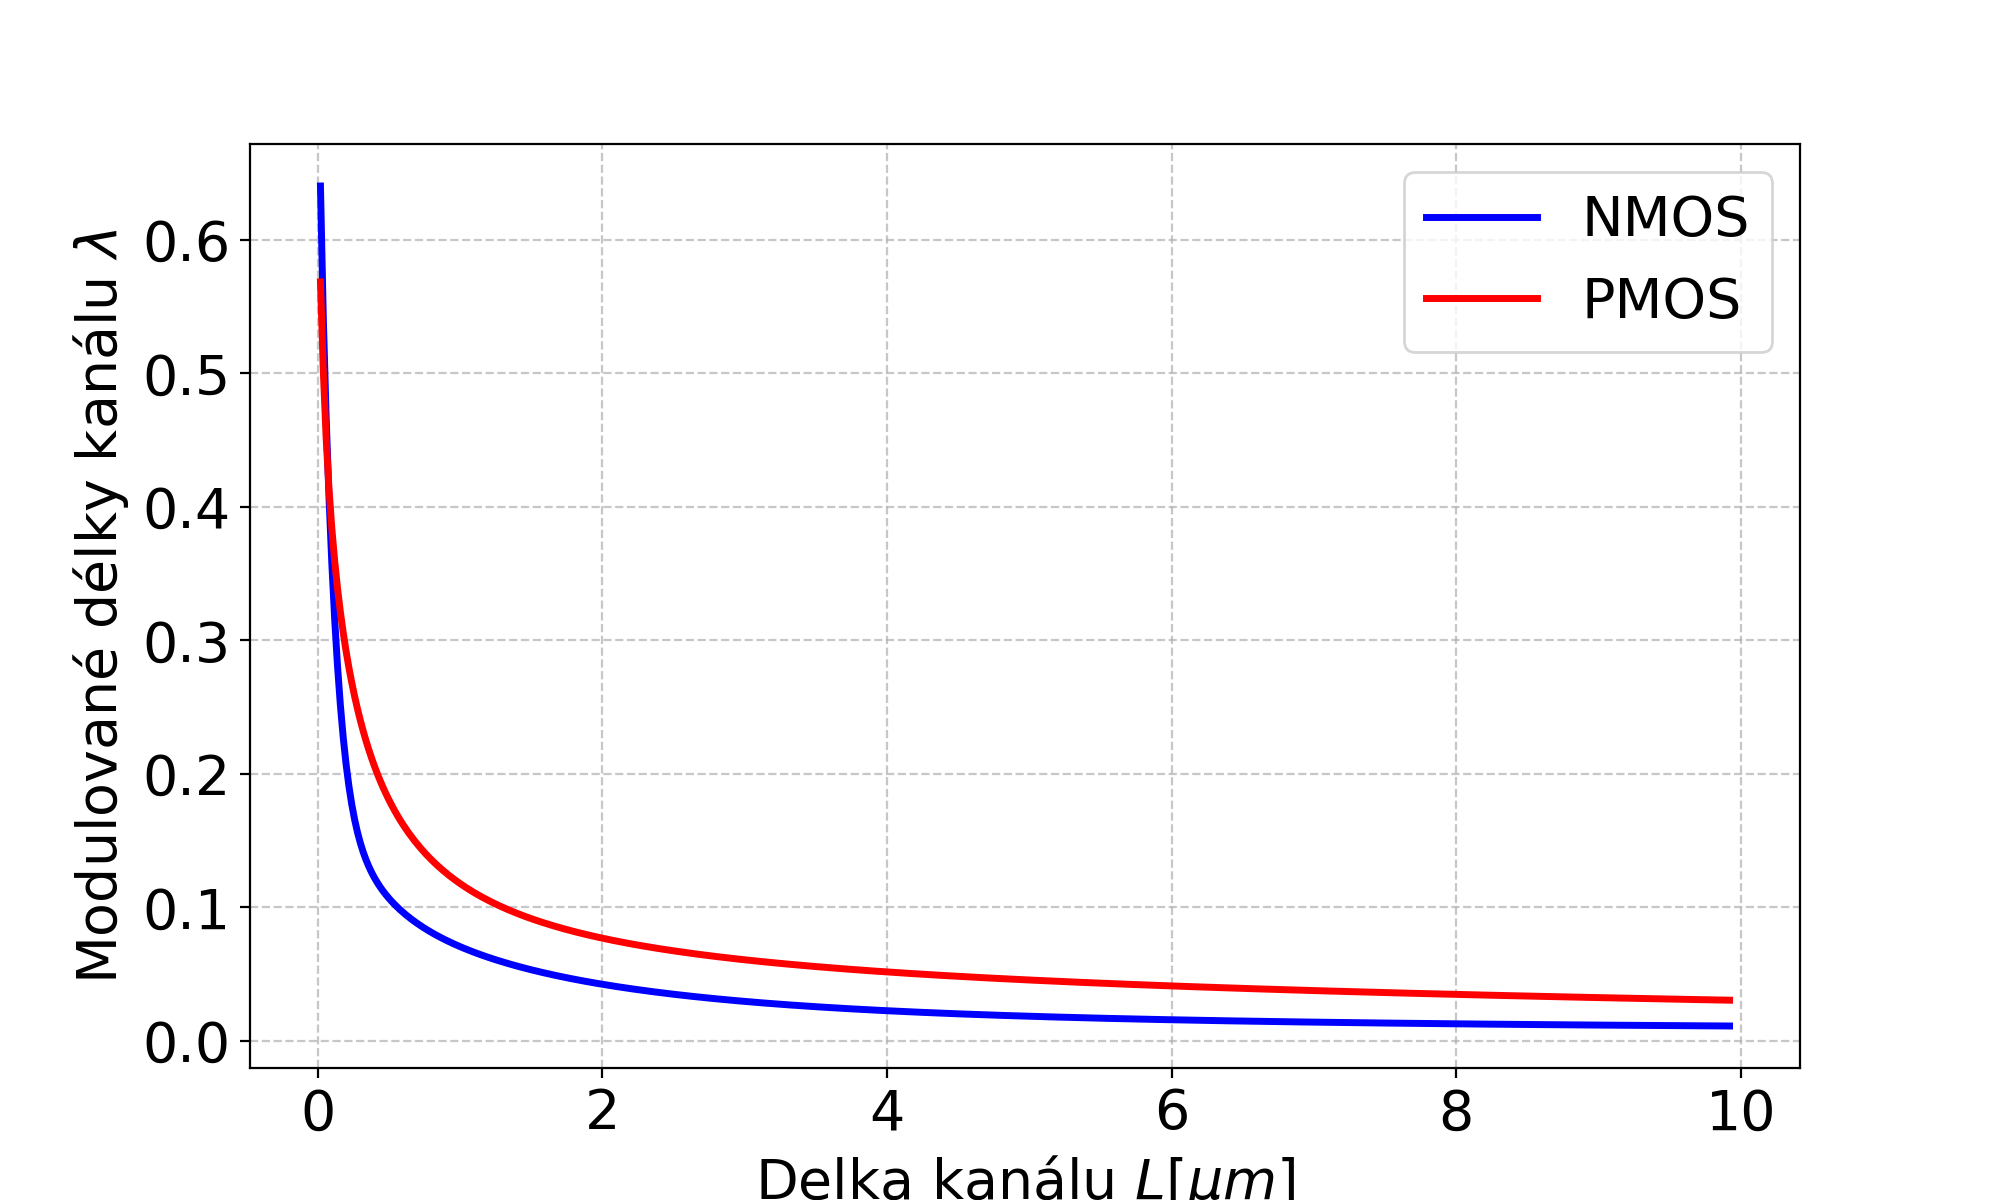
\includegraphics[height=0.28\textheight]{text/img/lambda.png}
    \caption{\label{fig:lambda} Závislost parametru \(\lambda\) na délce kanálu \(L\) při poměru \(W/L = 5\)}
\end{figure}

\vspace{-1mm}
\begin{figure}[H]
    \vspace{8mm}
    \begin{minipage}{0.5\textwidth}
        \begin{circuitikz}[scale=1, transform shape] 
            \draw
              % MOSFET transistor with labels for drain (D), gate (G), source (S), and bulk (B)
              (0,0) node[nmos, bulk] (mos) {}
              (mos.drain) node[left] {M1}
            
              % Gate voltage source VGS
              (mos.gate) to[short, -] ++(-2,0) to[voltage source, l^=$V_{GS}$] ++(0,-1.5) node[ground] {}
              
              % Drain voltage source VDS (vertical)
              (mos.drain) to[short, -] ++(0,1) -- ++(2,0) -- ++(0,-1) to[voltage source, l^=$V_{DS} $] ++(0,-2) -- (2,-1.5) node[ground] {}
              
              % Source connected to ground, aligned with VGS ground
              (mos.source) to[short, -] (0,-1.5) node[ground] {}
              
              % Bulk (body) connection to ground
              (mos.bulk) to[short, -] (0.5, 0) -- ++(0,-1) -- ++(-0.5,0)  node[circle,fill,inner sep=1pt] (myNode) {}
            ;
        \end{circuitikz}

        \vspace{5mm}
        \centering{(NMOS)}
    \end{minipage}
    \hfill
    \begin{minipage}{0.5\textwidth}
        \begin{circuitikz}[scale=1, transform shape] 
            \draw
              % MOSFET transistor with labels for drain (D), gate (G), source (S), and bulk (B)
              (0,0) node[pmos, bulk] (mos) {}
              (mos.drain) node[left] {M1}
                          
              % Gate voltage source VGS
              (mos.gate) to[short, -] (-2,0) to[voltage source, l^=$V_{GS}$] (-2,2) -- ++(2,0) node[circle,fill,inner sep=1pt] (myNode) {}
              
              % Drain voltage source VDS (vertical)
              (mos.source) to[short, -] (0,2) -- ++(2,0) -- ++(0,-1) to[voltage source, l^=$V_{DS} $] ++(0,-2) -- (2,-1.5) -- (0,-1.5)
              
              % Source connected to ground, aligned with VGS ground
              (mos.drain) to[short, ] (0,-1.5) node[circle,fill,inner sep=1pt] (myNode) {} (0,-1.5) node[ground] {}

              % Bulk (body) connection to ground
              (mos.bulk) to[short, -] (0.5, 0) -- ++(0,1) -- ++(-0.5,0)  node[circle,fill,inner sep=1pt] (myNode) {}

            %   (2,2)  to[short, *-o] ++(1,0) node[above, right]{$V_{CC}$}
            ;
        \end{circuitikz}

        \vspace{5mm} 
        \centering{(PMOS)}
    \end{minipage}
    \caption{\label{cod:cod_NP_WL_const} Zapojení pro určení závislosti modulace delky kanálu \(\lambda\) na delce kanálu \(L\)}
\end{figure}

\begin{lstlisting}[language=Spice, caption={ \centering Kod simulace použítí pro získání závislosti \\ modulované délky kanálu \(\lambda\) na délce kanálu \(L\)}, label={cod:cod_lambda}]
.lib cmos018.txt
.step param lset 0.1u 10u 0.02u
.param wset=5*lset
.meas DC ID1 FIND Id(M1) WHEN V(VD)=0.5
.meas DC ID2 FIND Id(M1) WHEN V(VD)=1.3
.meas DC ID0 FIND Id(M1) WHEN V(VD)=0.9
.meas rout param (1.3-0.5)/(ID2-ID1)
.meas lambda param 1/(ID0*rout)
.dc UDS 0.5 1.3 10m
\end{lstlisting}

\vspace{-7mm}
\begin{figure}[h]
    \centering
    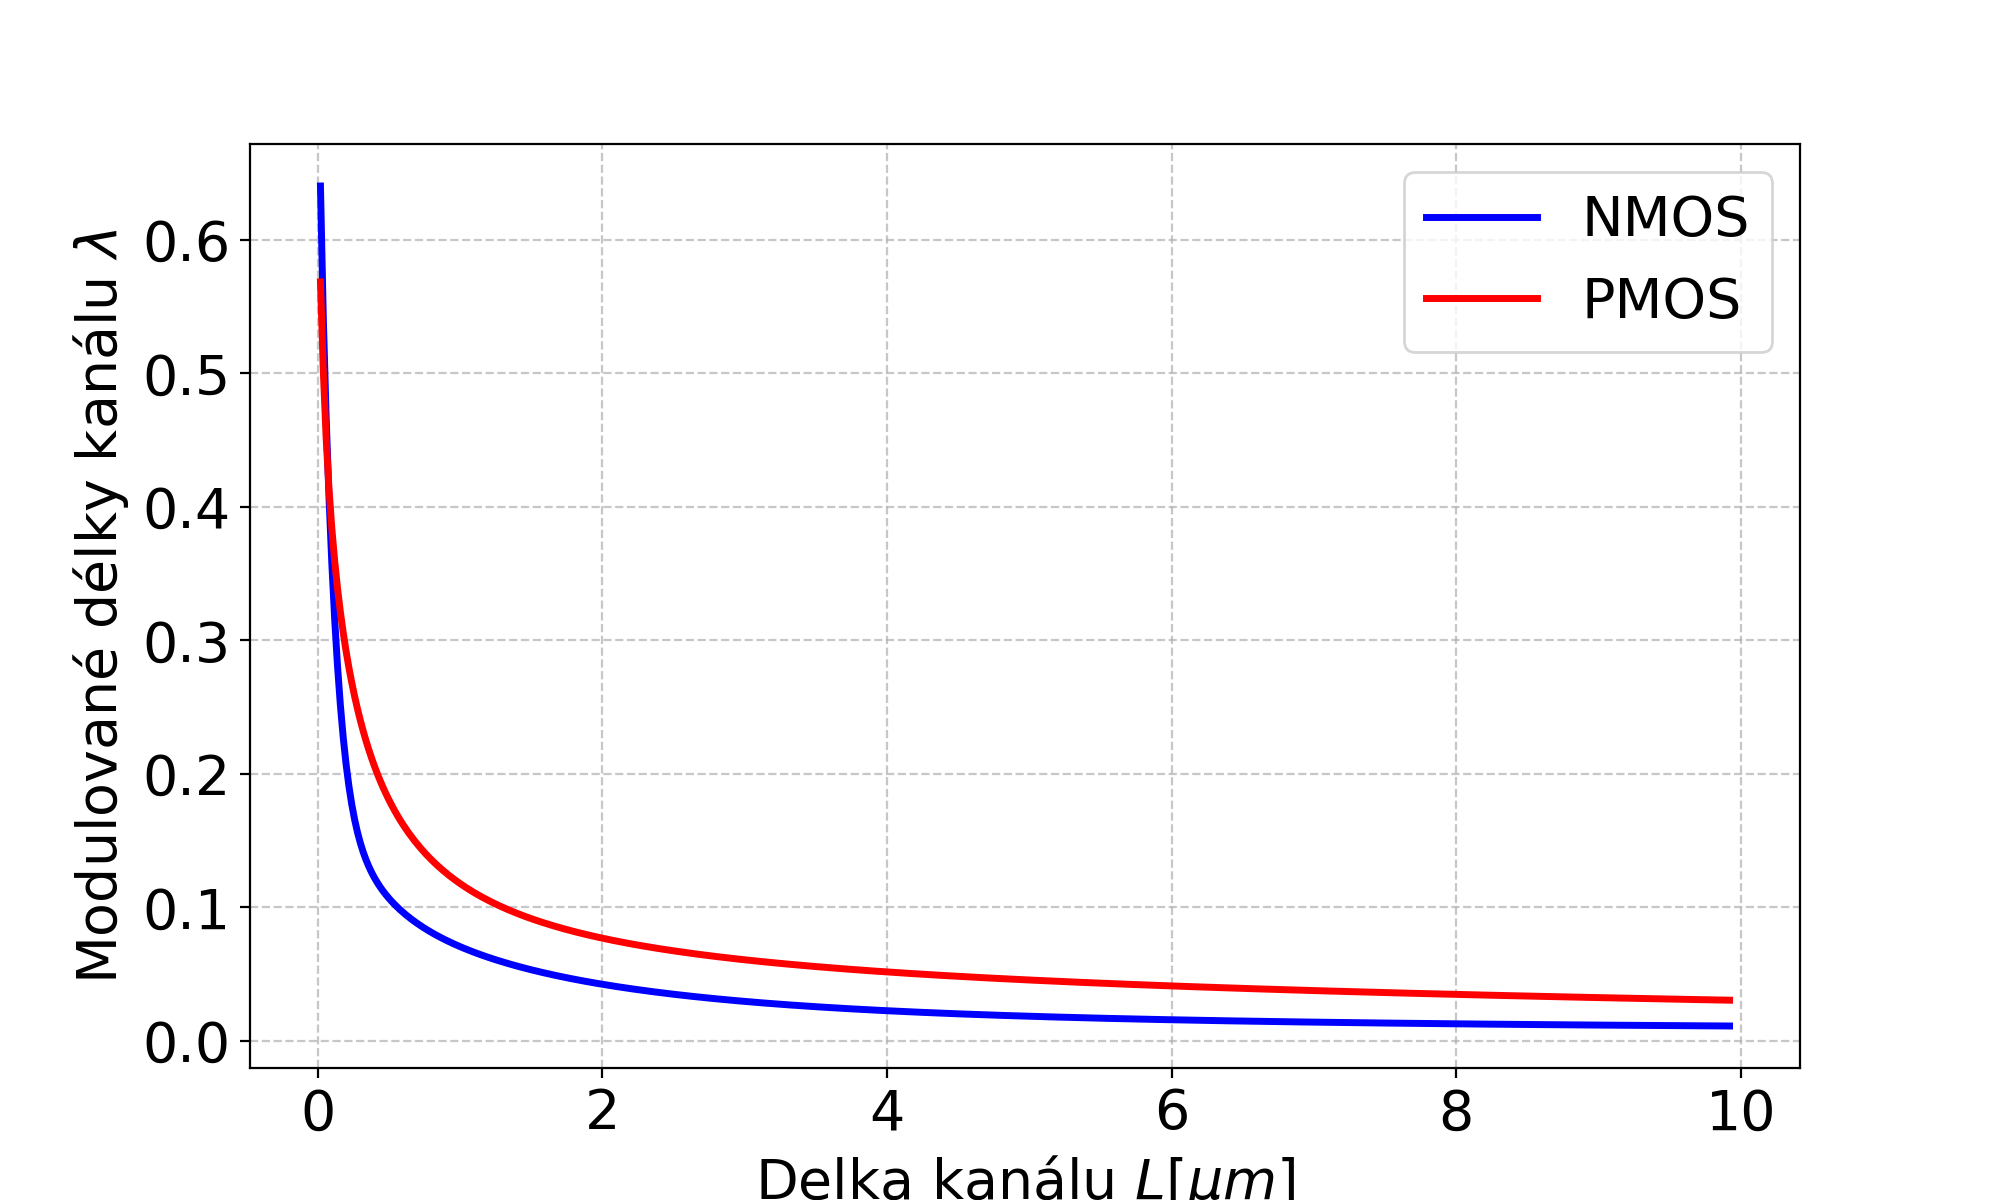
\includegraphics[height=0.28\textheight]{text/img/lambda.png}
    \caption{\label{fig:lambda} Závislost parametru \(\lambda\) na délce kanálu \(L\) při poměru \(W/L = 5\)}
\end{figure}

\vspace{-1mm}
\input{text/table/lambda.tex}



